\documentclass[tikz,border=10pt]{standalone}
\usepackage[T1]{fontenc}
\usepackage{lmodern}
\usetikzlibrary{arrows.meta,backgrounds,calc}
\definecolor{blue}{HTML}{0072B2}
\definecolor{orange}{HTML}{B44B00}
\definecolor{ink}{HTML}{243447}
\definecolor{gray}{HTML}{738294}
\tikzset{
 box/.style={draw=gray,rounded corners=3pt,text width=38mm,minimum height=17mm,align=center,text=ink,inner sep=6pt,font=\sffamily\small},
 skill/.style={box,fill=blue!6},
 external/.style={box,fill=gray!7},
 flow/.style={-{Latex[length=2.5mm]},draw=blue,line width=1.25pt},
 repair/.style={-{Latex[length=2.5mm]},draw=orange,line width=1.1pt},
 relation/.style={draw=gray,dashed,line width=.85pt},
 label/.style={font=\sffamily\small,text=ink,align=center},
 heading/.style={font=\sffamily\bfseries,text=ink,anchor=west},
 files/.style={font=\ttfamily\small,text=ink,anchor=north west,align=left},
 every node/.append style={font=\sffamily}
}
\newcommand{\step}[1]{\tikz[baseline=(s.base)]\node[circle,fill=blue,text=white,inner sep=2pt,font=\sffamily\tiny\bfseries](s){#1};}
\begin{document}
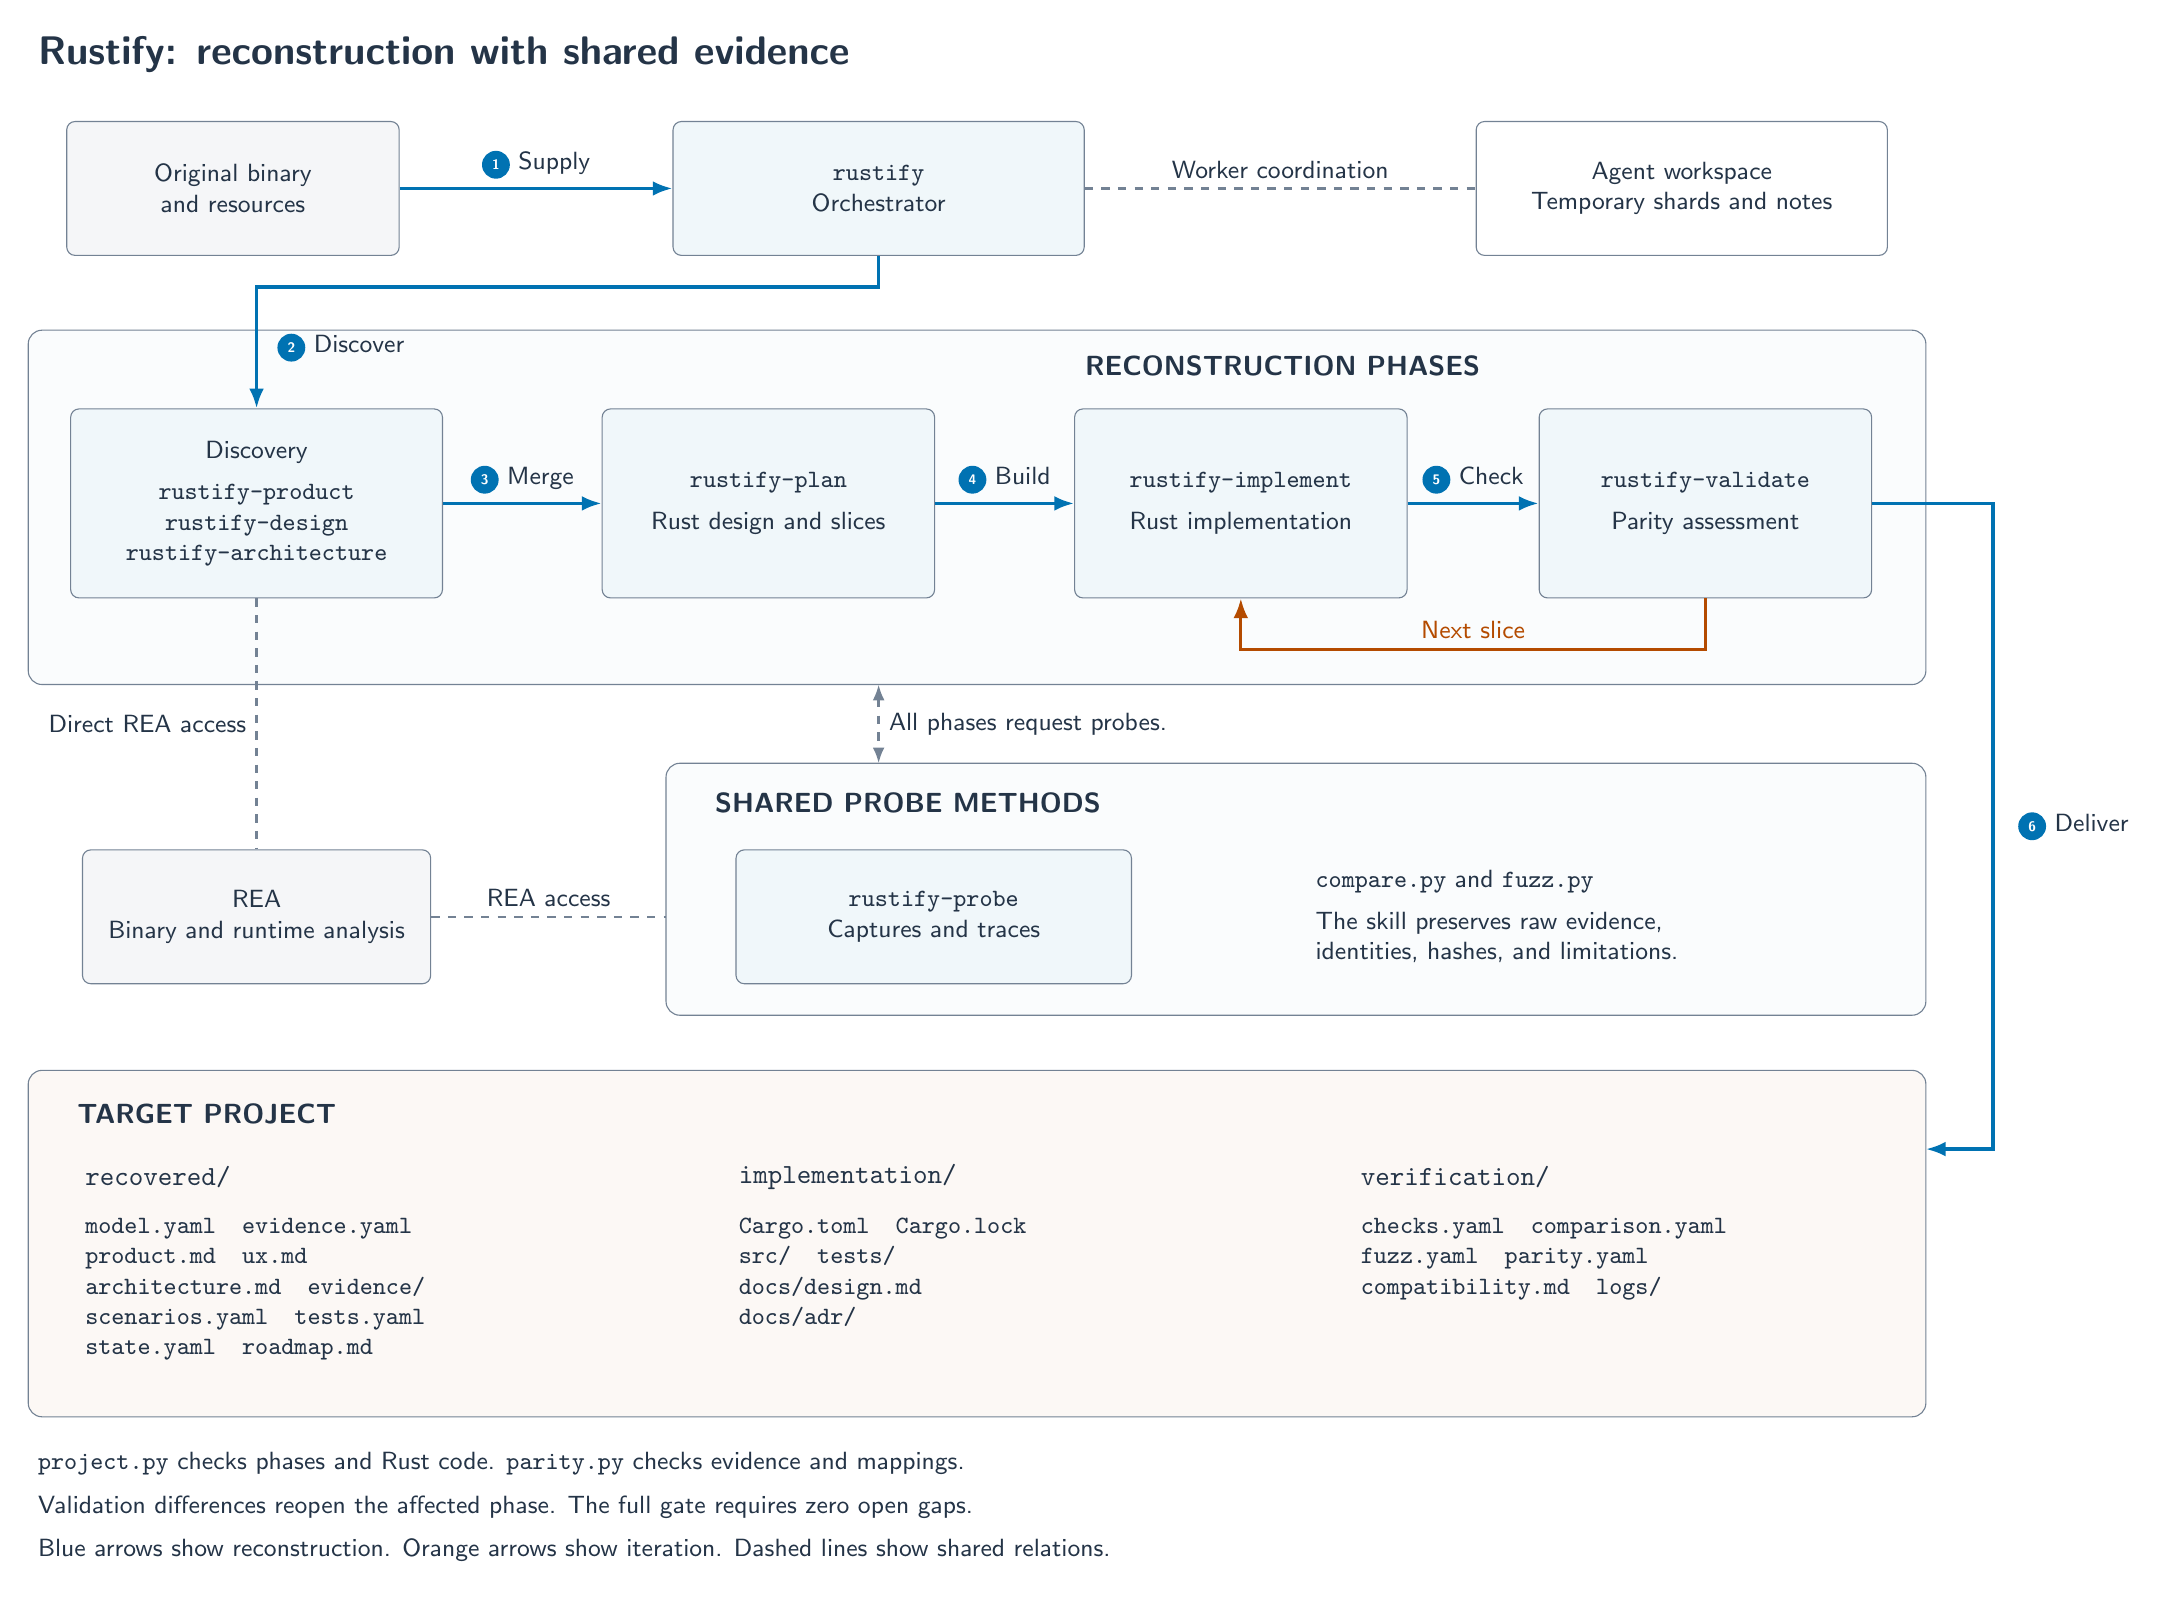
\begin{tikzpicture}[x=1cm,y=1cm]
 \node[heading,font=\sffamily\bfseries\Large] at (.2,17.6) {Rustify: reconstruction with shared evidence};
 \node[external] (input) at (2.8,15.9) {Original binary\\and resources};
 \node[skill,text width=48mm] (main) at (11.0,15.9) {\texttt{rustify}\\Orchestrator};
 \node[box,text width=48mm] (workspace) at (21.2,15.9) {Agent workspace\\Temporary shards and notes};
 \draw[flow] (input.east) -- node[label,above]{\step{1} Supply} (main.west);
 \draw[relation] (main.east) -- node[label,above]{Worker coordination} (workspace.west);
 \begin{scope}[on background layer]
  \filldraw[fill=blue!2,draw=gray,rounded corners=5pt] (.2,9.6) rectangle (24.3,14.1);
  \filldraw[fill=blue!2,draw=gray,rounded corners=5pt] (8.3,5.4) rectangle (24.3,8.6);
  \filldraw[fill=orange!4,draw=gray,rounded corners=5pt] (.2,.3) rectangle (24.3,4.7);
 \end{scope}
 \node[heading] at (13.5,13.65) {RECONSTRUCTION PHASES};
 \node[skill,text width=43mm,minimum height=24mm] (discovery) at (3.1,11.9) {Discovery\\[4pt]\texttt{rustify-product}\\\texttt{rustify-design}\\\texttt{rustify-architecture}};
 \node[skill,minimum height=24mm] (plan) at (9.6,11.9) {\texttt{rustify-plan}\\[4pt]Rust design and slices};
 \node[skill,minimum height=24mm] (implement) at (15.6,11.9) {\texttt{rustify-implement}\\[4pt]Rust implementation};
 \node[skill,minimum height=24mm] (validate) at (21.5,11.9) {\texttt{rustify-validate}\\[4pt]Parity assessment};
 \draw[flow] (main.south) -- (11.0,14.65) -- (3.1,14.65) -- node[label,right,xshift=4pt]{\step{2} Discover} (discovery.north);
 \draw[flow] (discovery.east) -- node[label,above]{\step{3} Merge} (plan.west);
 \draw[flow] (plan.east) -- node[label,above]{\step{4} Build} (implement.west);
 \draw[flow] (implement.east) -- node[label,above]{\step{5} Check} (validate.west);
 \draw[repair] (validate.south) -- (21.5,10.05) -- node[label,above,text=orange]{Next slice} (15.6,10.05) -- (implement.south);
 \node[heading] at (8.8,8.1) {SHARED PROBE METHODS};
 \node[skill,text width=46mm] (probe) at (11.7,6.65) {\texttt{rustify-probe}\\Captures and traces};
 \node[label,text width=61mm,align=left] at (19.6,6.65) {\texttt{compare.py} and \texttt{fuzz.py}\\[4pt]The skill preserves raw evidence,\\identities, hashes, and limitations.};
 \draw[relation,{Latex[length=2mm]}-{Latex[length=2mm]}] (11.0,9.6) -- node[label,right]{All phases request probes.} (11.0,8.6);
 \node[external,text width=40mm] (rea) at (3.1,6.65) {REA\\Binary and runtime analysis};
 \draw[relation] (discovery.south) -- node[label,left]{Direct REA access} (rea.north);
 \draw[relation] (rea.east) -- node[label,above]{REA access} (8.3,6.65);
 \node[heading] at (.7,4.15) {TARGET PROJECT};
 \node[heading,font=\ttfamily\bfseries] at (.8,3.35) {recovered/};
 \node[files] at (.8,2.95) {model.yaml\quad evidence.yaml\\product.md\quad ux.md\\architecture.md\quad evidence/\\scenarios.yaml\quad tests.yaml\\state.yaml\quad roadmap.md};
 \node[heading,font=\ttfamily\bfseries] at (9.1,3.35) {implementation/};
 \node[files] at (9.1,2.95) {Cargo.toml\quad Cargo.lock\\src/\quad tests/\\docs/design.md\\docs/adr/};
 \node[heading,font=\ttfamily\bfseries] at (17.0,3.35) {verification/};
 \node[files] at (17.0,2.95) {checks.yaml\quad comparison.yaml\\fuzz.yaml\quad parity.yaml\\compatibility.md\quad logs/};
 \draw[flow] (validate.east) -- (25.15,11.9) -- node[label,right,text width=18mm]{\step{6} Deliver} (25.15,3.7) -- (24.3,3.7);
 \node[label,anchor=west] at (.2,-.3) {\texttt{project.py} checks phases and Rust code. \texttt{parity.py} checks evidence and mappings.};
 \node[label,anchor=west] at (.2,-.85) {Validation differences reopen the affected phase. The full gate requires zero open gaps.};
 \node[label,anchor=west] at (.2,-1.4) {Blue arrows show reconstruction. Orange arrows show iteration. Dashed lines show shared relations.};
\end{tikzpicture}
\end{document}
